\documentclass{anstrans}
%%%%%%%%%%%%%%%%%%%%%%%%%%%%%%%%%%%
\title{Dynamic Resource Exchange Performance in Cyclus}
\author{Matthew J.~Gidden, Paul P. H.~Wilson}

\institute{
University of Wisconsin, Madison WI
}

\email{gidden@wisc.edu}

%%%% packages and definitions (optional)
\usepackage{graphicx} % allows inclusion of graphics
\usepackage{booktabs} % nice rules (thick lines) for tables
\usepackage{microtype} % improves typography for PDF

\usepackage{multirow} % combining rows in tables
\usepackage{tabularx} % for tables with line breaks

\newcommand{\Cyclus}{\textsc{Cyclus}}
\newcommand{\ffc}{$f_{\text{fc}}$}
\newcommand{\frx}{$f_{\text{rx}}$}
\newcommand{\floc}{$f_{\text{loc}}$}

\begin{document}

%%%%%%%%%%%%%%%%%%%%%%%%%%%%%%%%%%%%%%%%%%%%%%%%%%%%%%%%%%%%%%%%%%%%%%%%%%%%%%%%
\section{Introduction}
Nuclear fuel cycle simulation (FCS) is a field which seeks to model the
facilities and material flows required to produce nuclear power. Simulations
normally model a time span decades, or even centuries. Furthermore, myriad
decisions exist within a given fuel cycle simulation, such as the deployment
timing of facility types and deciding how material transfers should be executed
at a given time step. Accordingly, tradeoffs exist between the features provided
by a simulator and the performance of the simulator.

The \Cyclus{} FCS \cite{cyclus2014} was designed to more easily model a variety
of fuel cycles. It uses an agent-based modeling paradigm in order to encapsulate
the difficulty of designing new agent archetypes. Archetypes define
parameterized agent logic and behavior, and can therefore be reused within and
between simulations. The core agent-interaction model in \Cyclus{} is the
Dynamic Resource Exchange (DRE) \cite{gidden_agent-based_2013,
  gidden_agent-based_2014}. The DRE, recomputed at each time step, polls the
supply and demand of commodities in the simulation and then determines the
trades to be executed between agents. Coupling the DRE with the \Cyclus{}
Region-Institution-Facility hierarchy model as well as the
archetype-prototype-agent model, highly dynamic, easily adjustable fuel cycles
can be modeled, addressing many of the issues developers and users have found
with previous models. However, \Cyclus{} must both be featureful and
performant. This paper provides a first-look at how the DRE model, also called
the Nuclear Fuel Cycle Transportation Problem (NFCTP), scales with problem size
by generating and solving a large number of exchanges. Different solvers are
analyzed including a \Cyclus{}-aware greedy heuristic in addition to COIN-OR's
LP and MILP solvers \cite{coinclp, coincbc}.

%%%%%%%%%%%%%%%%%%%%%%%%%%%%%%%%%%%%%%%%%%%%%%%%%%%%%%%%%%%%%%%%%%%%%%%%%%%%%%%%
\section{Methodology}

Instances of resource exchanges are required to analyze the effects and
performance of the NFCTP formulation and its solvers. In the absence of large
Cyclus simulations with interesting facility and relationship models, instances
must be generated given some set of rules and parameters. Two distinct
\textit{species} of exchanges are generated, those related to the \textit{front
  end} of the nuclear fuel cycle and those related to the \textit{back end} of
the nuclear fuel cycle. For each species, commodities, reactors, and supporting
facilities must be generated in addition to exchange-related parameters, such as
the trade preferences.

Three types of fuel cycles can be generated: a once-through fuel cycle, labeled
OT; a plutonium-recycle fuel cycle, labeled MOX; and a plutonium and
thorium-recycle fuel cycle, labeled MOX-ThOX. As fuel cycles increase in
complexity, the number of commodities that exist increases, as shown in Table
\ref{tbl:fc_to_commods}. The commodities are referred to by abbreviation:
Uranium Oxide (UOX), Mixed Plutonium Oxide for Thermal Reactors (TMOX), Mixed
Plutonium Oxide for Fast Reactors (FMOX), Thorium Oxide for Fast Reactors
(FThOX).

\begin{table}[]
\centering
\caption{A mapping between fuel cycles to the commodities that exist in each one.}
\label{tbl:fc_to_commods}
\begin{tabular}{|c|c|}
\hline
\textbf{Fuel Cycle}            & \textbf{Commodities} \\ \hline
OT                    & UOX         \\ \hline
\multirow{3}{*}{MOX}  & UOX         \\  
                      & TMOX        \\  
                      & FMOX        \\ \hline
\multirow{4}{*}{ThOX} & UOX         \\  
                      & TMOX        \\  
                      & FMOX        \\  
                      & FThOX       \\ \hline
\end{tabular}
\end{table}

All reactors are modeled as either thermal or fast reactors. It is necessary to
estimate the amount of fuel exchanged by reactors each time step. Accordingly,
thermal reactors are simplified models of AP-1000 reactors, and fast reactors
are simplified models of BN-600 reactors. Reactors operate in a batch mode,
where each batch is approximately one quarter of the reactor core, an assumption
which similar to other analyses \cite{rineiski2011reactivity}. Each reactor in
the exchange is either offering or requesting a batch of fuel. Reactors may be
fueled by different fuel types, i.e., fuel commodities. A mapping of reactors to
acceptable commodities is provided in Table \ref{tbl:rx_to_commods}. Note that
there is still a preference distribution associated with each reactor-commodity
pair as well as constraint coefficient effects.

\begin{table}[]
\centering
\caption{A mapping between reactor types and the commodities allowed to fuel 
  each reactor type.}
\label{tbl:rx_to_commods}
\begin{tabular}{|c|c|}
\hline
\textbf{Reactor Types}            & \textbf{Fuel Commodities} \\ \hline
\multirow{3}{*}{Thermal}                    & UOX         \\ 
                      & TMOX        \\  
                      & FMOX       \\ \hline
\multirow{4}{*}{FMOX}  & UOX         \\  
                      & TMOX        \\ 
                      & TMOX        \\  
                      & FThOX        \\ \hline 
\multirow{4}{*}{FThOX} & UOX         \\  
                     & TMOX        \\ 
                      & TMOX        \\  
                      & FThOX        \\ \hline 
\end{tabular}
\end{table}

In a front-end exchange, fuel suppliers exchange material with reactors. In a
back-end exchange, reprocessing and storage facilities exchange material with
reactors. In either case, facilities that are \text{not} reactors are referred
to as \textit{support} facilities, as they support the reactors which generate
power. In the front-end exchange model, a single type of supporting facility
exists for each fuel type, e.g., an enrichment facilit for UOX, a thermal
reprocessing plant for TMOX, etc. In the back-end exchange model, a similar
supporting facility distribution is used, except a storage facility type,
capable of storing any commodity is added.

For both reactors and support facilities in both exchange species, exchange
constructs, such as preferences and constraint coefficients, must be
generated. Constraint coefficients are a function of resource quality, for which
a proxy must be assigned. Accordingly, each reactor is modeled using an
enrichment-level-range-to-commodity mapping. For example, LWRs requesting UOX
have an enrichment range of $[3.5, 5.5]$. The enrichment value for each reactor
is chosen from a uniform distribution in order to differentiate
reactors. Preferences in the DRE are requester-based, and are assigned
per-commodity to requesters in both exchange species. In order to differentiate
between preferences, facilities are assigned a location proxy. The location
proxy can provide additional weight to preference values.

Exchange generation is parameterized and thus depends on a parameter
vector. While each species has specific parameters, both species share some
fundamental parameters, namely: which fuel cycle is being generated, whether
reactors are modeled using a single batch or a collection of assemblies, and to
what degree location is used in determining preference coefficients. Because
each parameter deals with a notion of simulation \textit{fidelity}, they are
denoted as $f_{x}$ and summarized in Table \ref{tbl:global_params}.

\begin{table}[]
\centering
\caption{Parameter Description Summary for Species-Independent Parameters.}
\label{tbl:global_params}
\begin{tabularx}{\columnwidth}{|c|X|c|} % line wraps second column if too long
\hline
Parameter    & 
Description & 
Values
\\ \hline
\ffc      &
Which fuel cycle is being modeled &
OT, MOX, THOX
\\ \hline
\frx    &
Whether individual assemblies are modeled or whole batches are modeled &
Batch, Assembly  
\\ \hline
\floc     &
To what degree is facility location included in objective coefficients &
None, Coarse, Fine
\\ \hline
\end{tabularx}
\end{table}

\begin{figure*}
  \begin{center}
    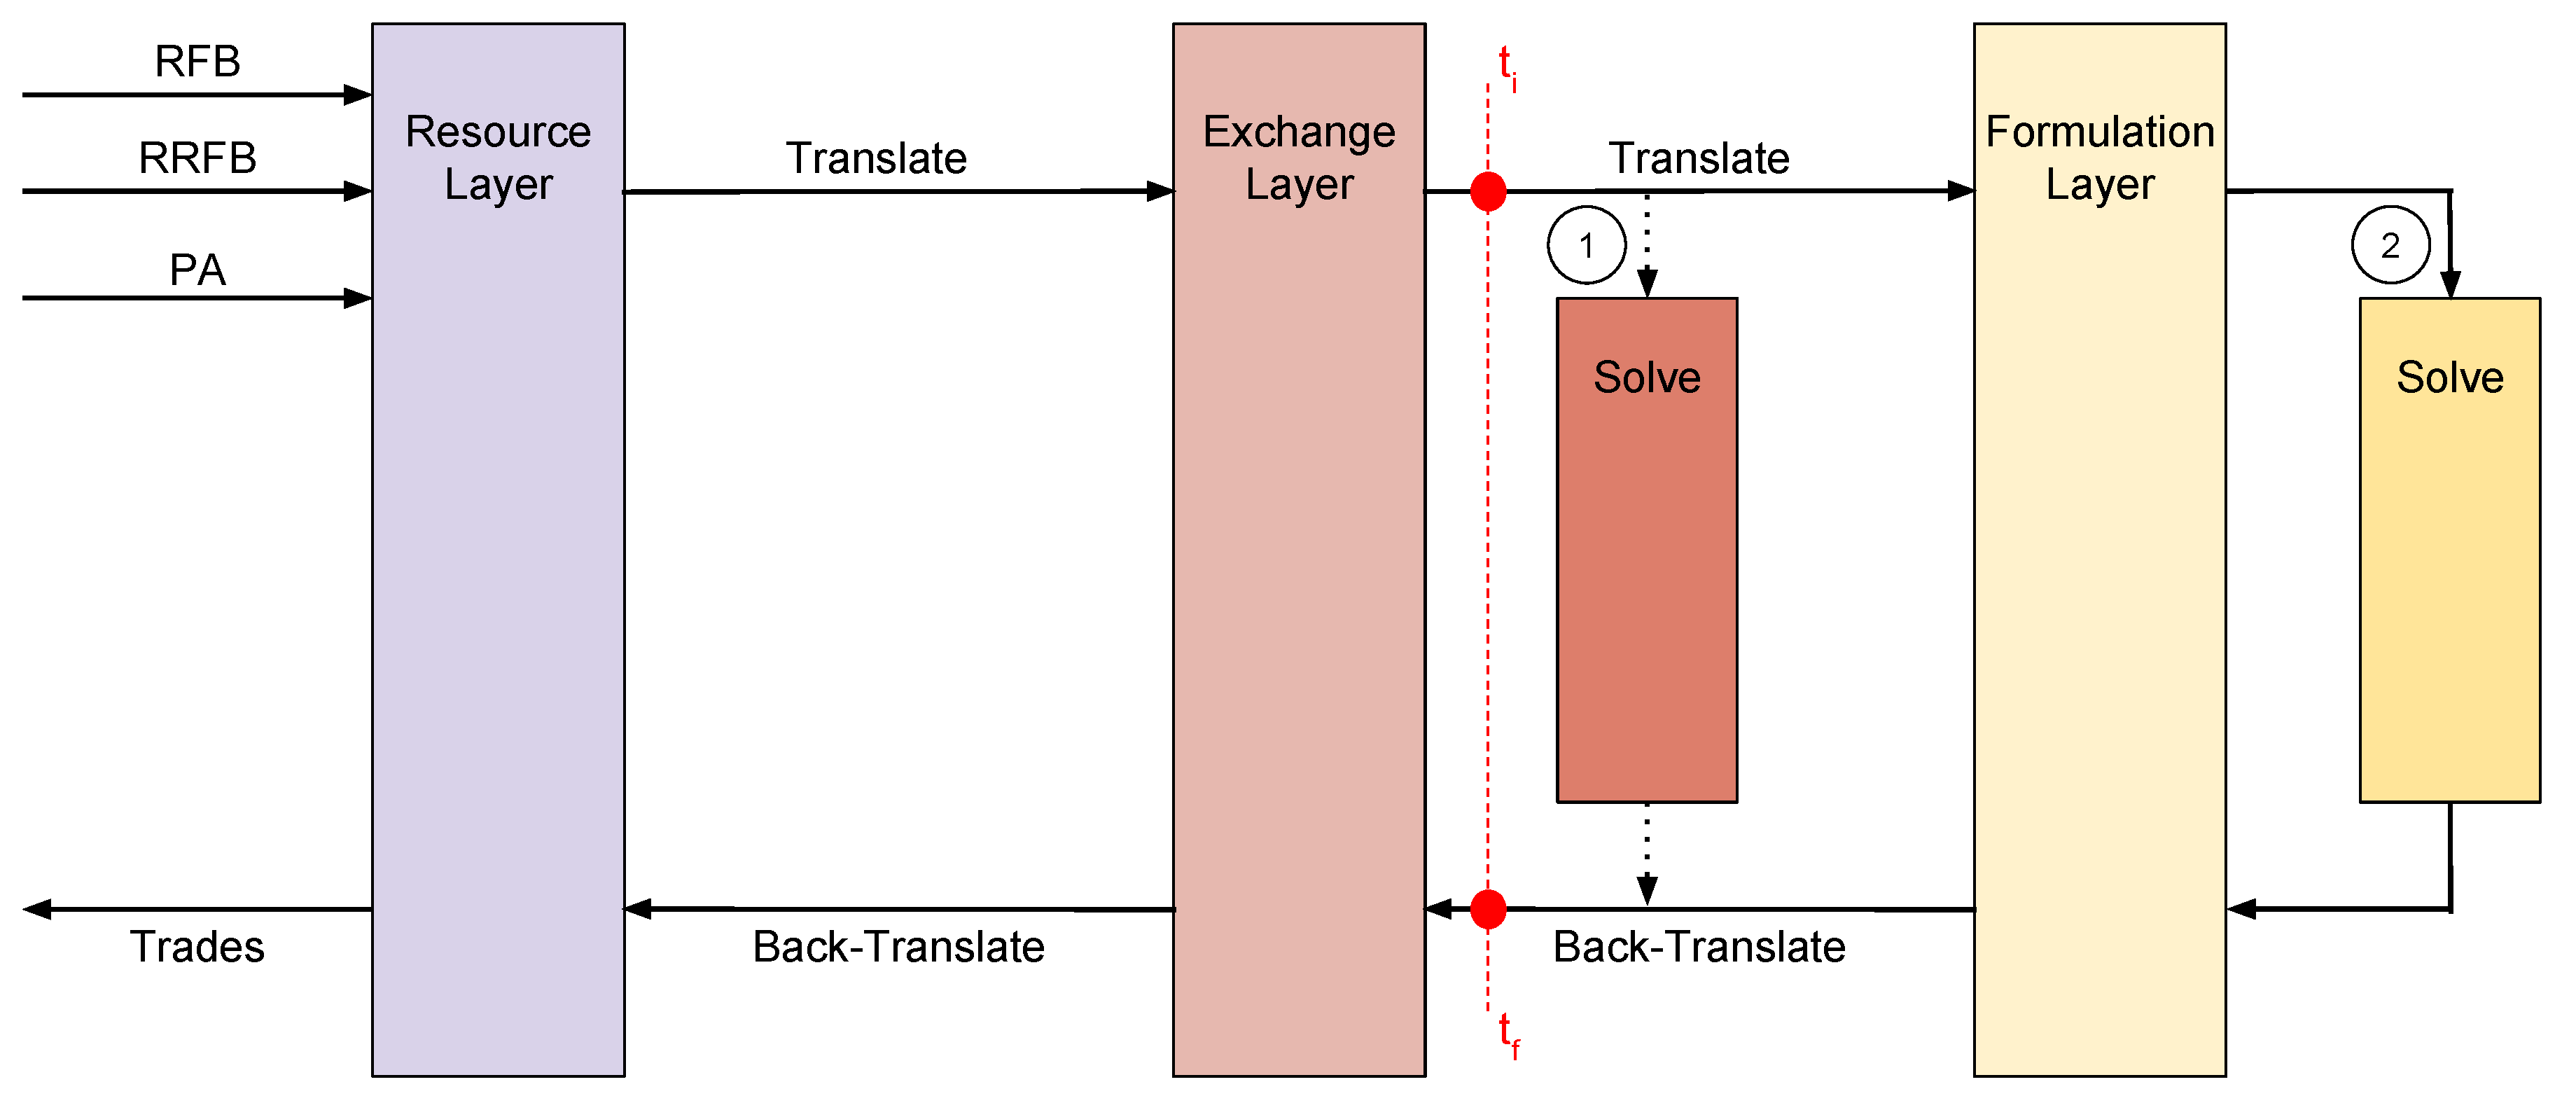
\includegraphics[width=2\columnwidth]{exchange_xlation_timing.pdf}
    \caption[]{
      \label{fig:dre_time}
      The control flow of the DRE execution and time points for comparing 
      different solutions. The DRE workflow is described more fully in 
      \cite{gidden_agent-based_2013, gidden_agent-based_2014}. }
  \end{center}
\end{figure*}

Given a set of parameters, an exchange instance is generated and persisted in a
database. The generated exchange exists in the \textit{exchange layer} of the
DRE, as shown in Figure \ref{fig:dre_time}. Because the greedy heuristic is
knowledgeable of \Cyclus, it uses solution pathway $1$ shown in the figure. The
COIN solvers must have the \Cyclus exchange structure formulated into a
mathematical program, described previously in \ref{gidden_agent-based_2013}, and
thus must take the second solver pathway, through the formulation layer. Figure
\ref{fig:dre_time} also notes the time points measured during execution in order
to compare solution times between solvers and different exchange instances,
i.e., for each solver and exchange instance, execution time is measured as $t_f
- t_i$.

In order to explore the large number of possible exchange instances, a
sophisticated instance generation and solving framework is needed. Accordingly,
a new software package called Cyclopts (\underline{Cycl}us
\underline{Opt}imization \underline{S}tudies) was developed. Cyclopts provides a
general framework for sampling a parameter space, defining problem instances for
a given point in parameter space, and solving a problem instance under a variety
of conditions. Cyclopts leverages an HTCondor-aware High Throughput Computing
(HTC) framework at UW-Madison in order to efficiently run exchange instances. 


%%%%%%%%%%%%%%%%%%%%%%%%%%%%%%%%%%%%%%%%%%%%%%%%%%%%%%%%%%%%%%%%%%%%%%%%%%%%%%%%
\section{Results and Analysis}

An experiment consists of a set of resource-exchange graph instances executed
with a collection of configured solvers. When a solution is found, the solution
(i.e., the flow vector), the time required to reach the solution, and the
objective value (i.e., the dot-product of cost and flow vectors) are
recorded. Six execution nodes on UW-Madison Advanced Computing Initiative (ACI)
HTCondor system form the homogeneous environment used to conduct the experiments
herein described. Each execute node is comprised of an 2.90 GHz eight-core,
sixteen-thread, Intel Xeon E5-2690 processor with 128 GB of RAM. Processor
hyper-threading was disabled for the duration of the experimental campaign to
allow comparisons between solution times.

Initially, a scalability campaign was launched to study how the solvers perform
as the size of exchange increases. All parameters for generating an exchange are
a function of the number of reactors in the exchange, thus the number of
reactors in the system is the natural choice for a scaling parameter. The number
of reactors in the system was scaled from ten to five hundred. For each reactor
population value, exchanges were generated for all possible combinations of
fundamental parameter values ($18$ total). Further, each generated exchange
instance was solved with all three available solvers. Figure
\ref{fig:greedy_size} provides an example of output from the scalability
campaign.

\begin{figure*}
  \begin{center}
    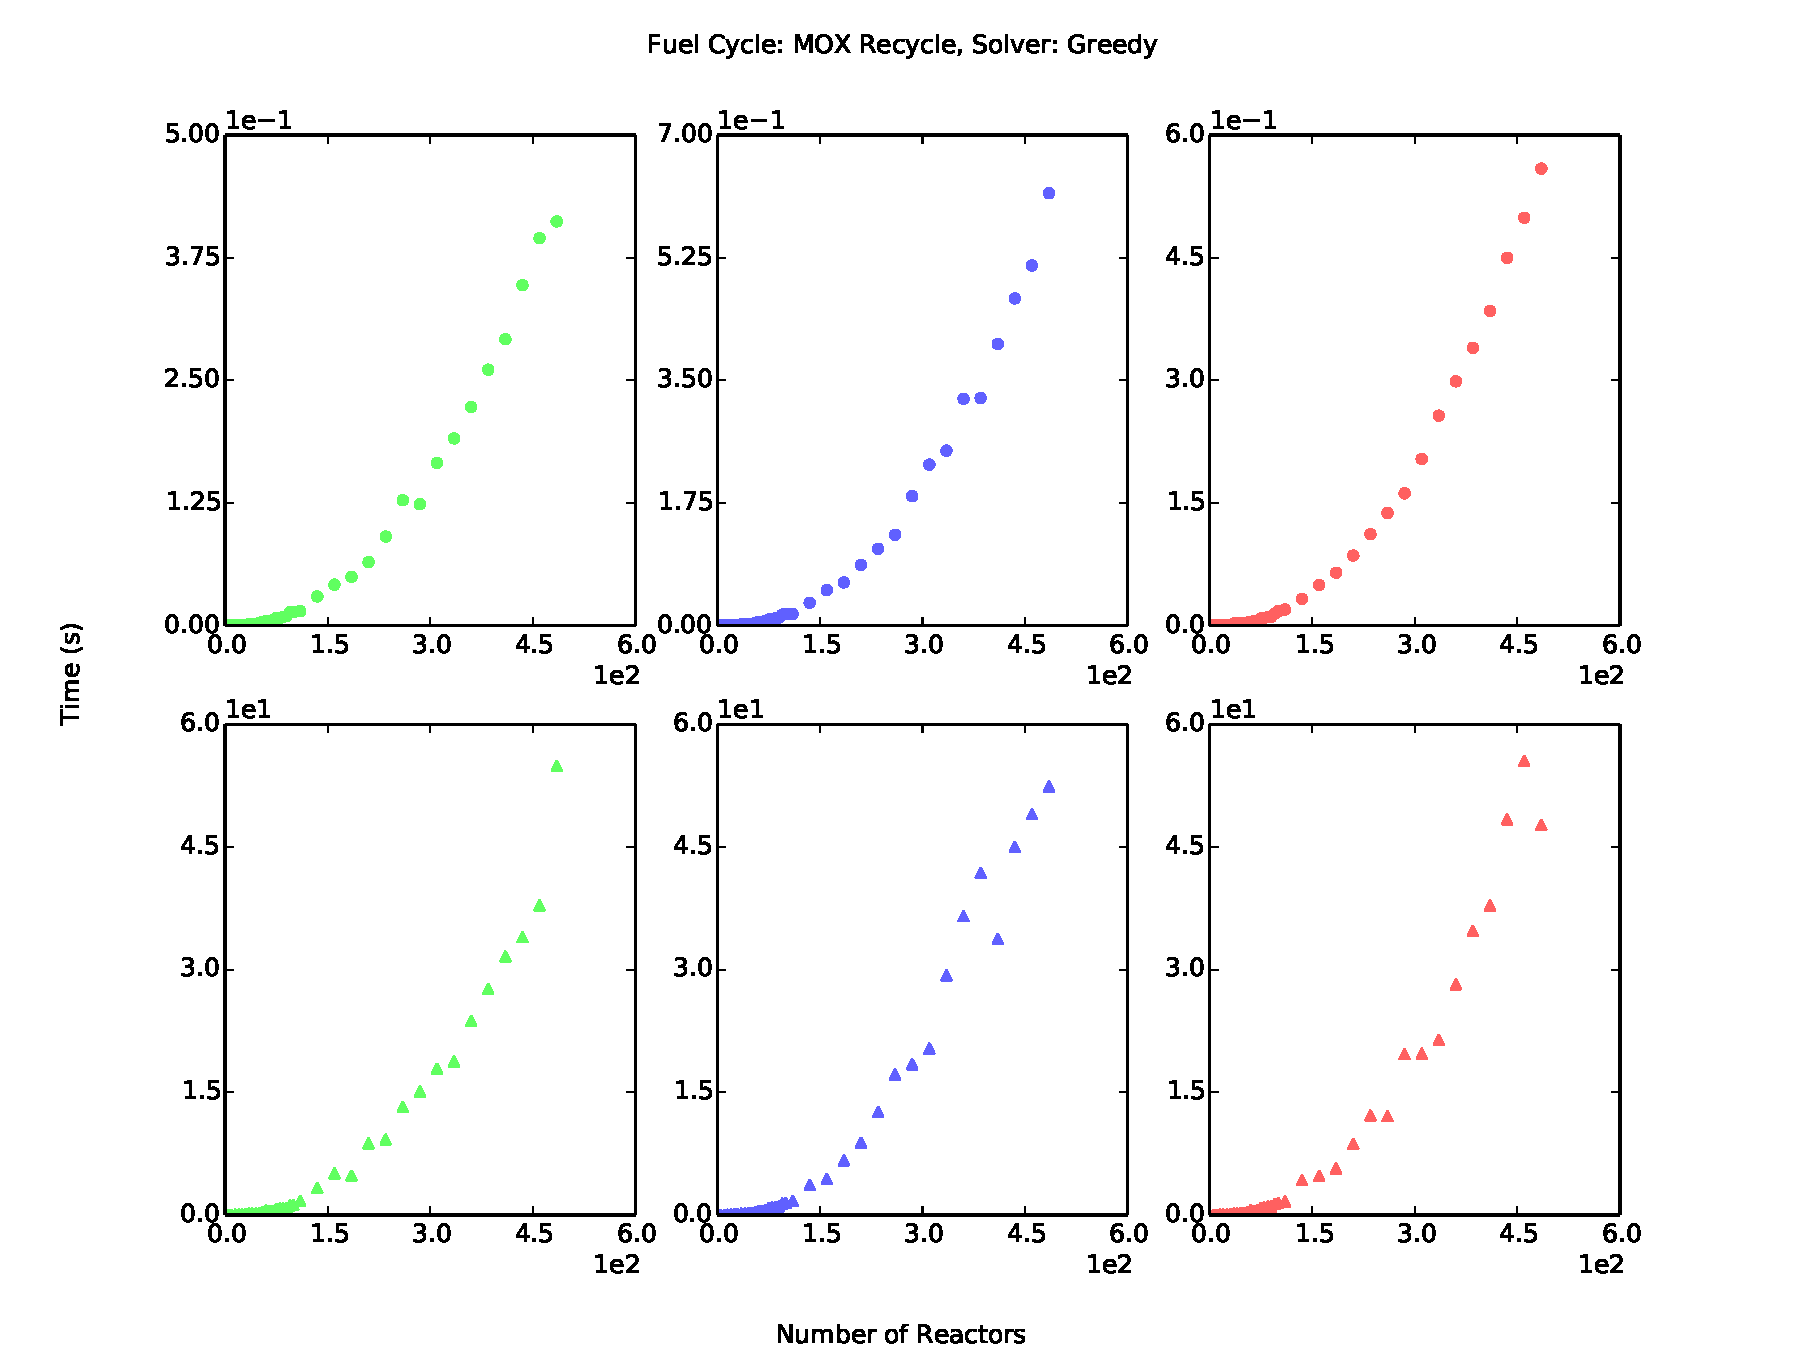
\includegraphics[width=1.5\columnwidth]{base_back_n_rxtr_time_fc1_solvergreedy.pdf}
    \caption[]{
      \label{fig:greedy_size}
      Results for the size scoping study for the greedy heuristic.
      }
  \end{center}
\end{figure*}

Every exchange instance depends on both objective value coefficients and
constraint coefficients, both of which are products of stochastic
processes. Accordingly, an experimental campaign was launched to study the
effects of stochasticity on the solution times and relative solution values
between solvers. Similar to the scalability campaign, all possible combinations
of fundamental parameter values were investigated; $1,000$ were generated as a
base line case study for each combination. Figure \ref{fig:cbc_stochastic}
provides an example of output from the stochastic campaign.

\begin{figure*}
  \begin{center}
    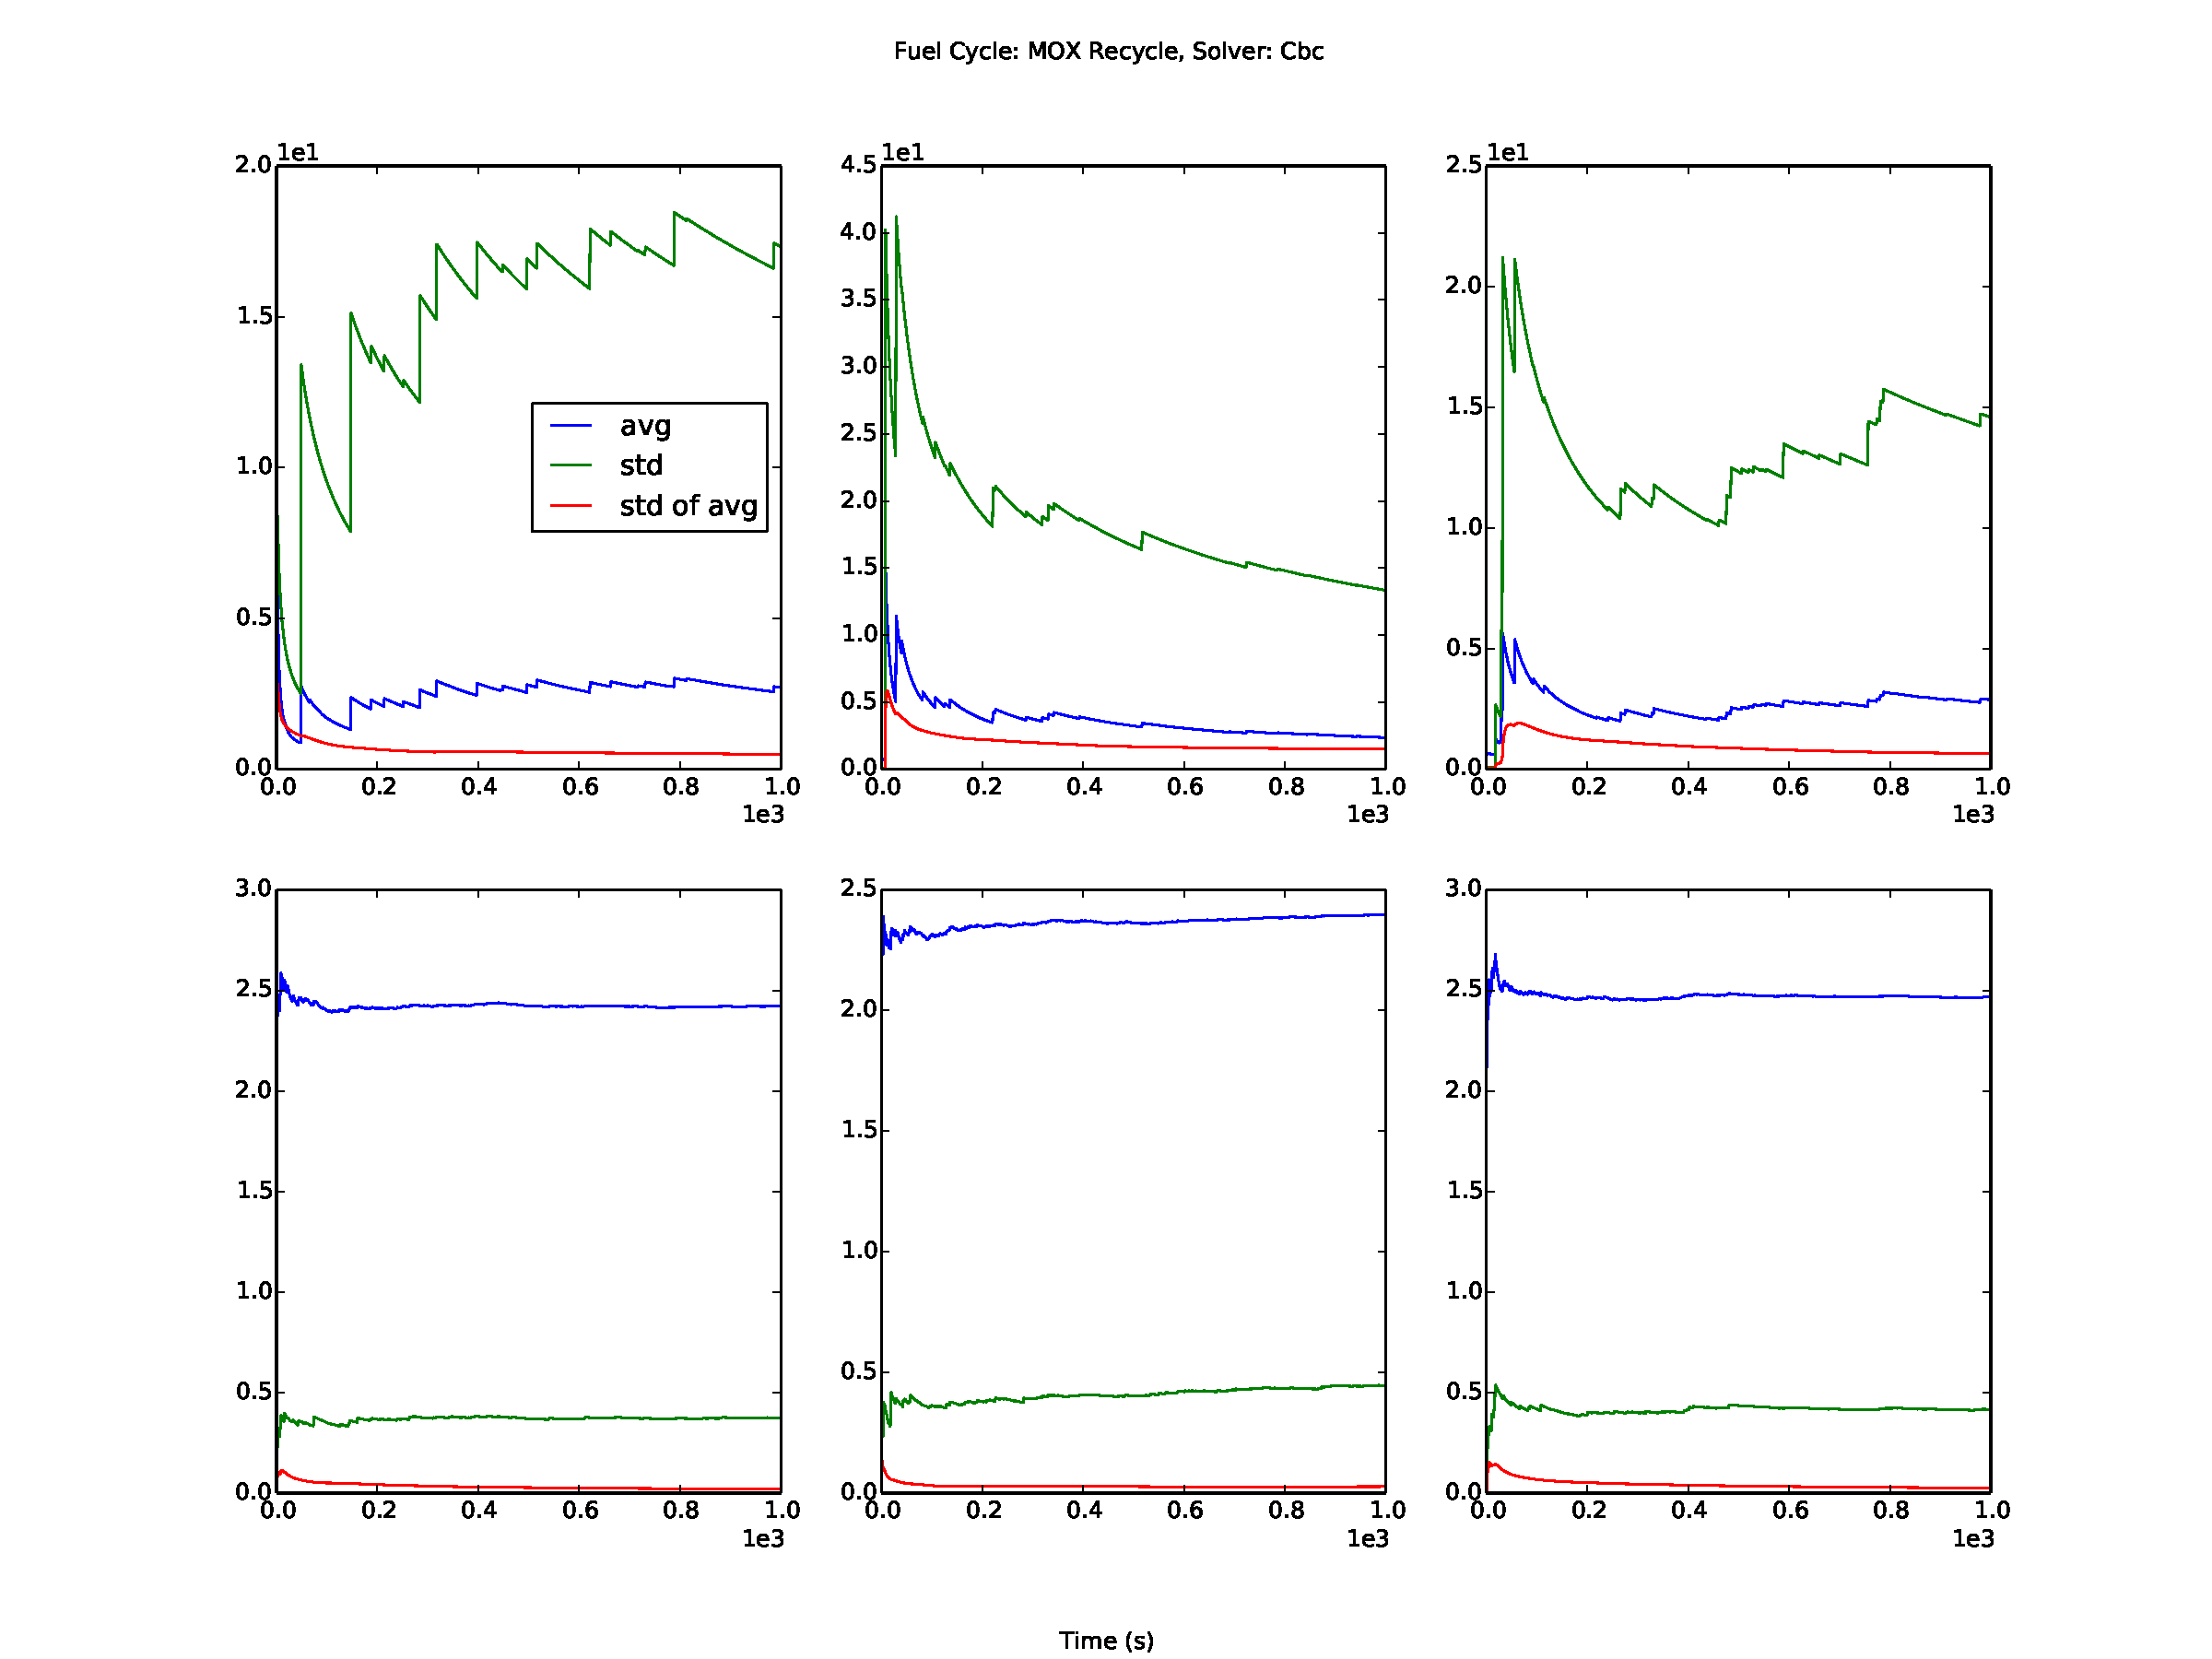
\includegraphics[width=1.5\columnwidth]{1k_avg_front_time_fc1_solvercbc.pdf}
    \caption[]{
      \label{fig:cbc_stochastic}
      Results for the size stochastic study for the CBC Solver.
      }
  \end{center}
\end{figure*}

%%%%%%%%%%%%%%%%%%%%%%%%%%%%%%%%%%%%%%%%%%%%%%%%%%%%%%%%%%%%%%%%%%%%%%%%%%%%%%%%
\section{Conclusions}


Conclusions

%%%%%%%%%%%%%%%%%%%%%%%%%%%%%%%%%%%%%%%%%%%%%%%%%%%%%%%%%%%%%%%%%%%%%%%%%%%%%%%%
\section{Acknowledgments}

This research is being performed using funding received from the DOE
Office of Nuclear Energy's Nuclear Energy University Programs.  The
authors thank the NEUP for its generous support.

\begin{center}

\includegraphics[width=.25\columnwidth]{neup_logo_large.jpg}
\end{center}

The authors would also like to thank Dr. Anthony M. Scopatz, whose advice in the
development of Cyclopts has proved invaluable.

%%%%%%%%%%%%%%%%%%%%%%%%%%%%%%%%%%%%%%%%%%%%%%%%%%%%%%%%%%%%%%%%%%%%%%%%%%%%%%%%
\bibliographystyle{ans}
\bibliography{bibliography}
\end{document}

